\documentclass[../main.tex]{subfiles}
\graphicspath{{\subfix{../images/}}}
\begin{document}
\label{Ex:Equi}
\index{exercises!equilibrium}

Keep the focus of your concentration on your center.

\noindent
\begin{tabular}{p{3cm} p{9cm} }
 \raisebox{-1.4\totalheight}{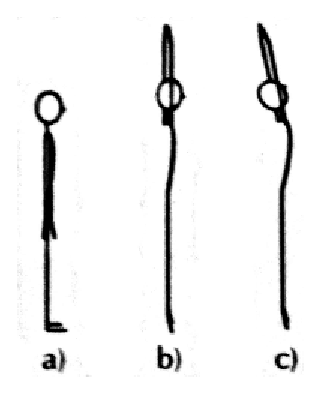
\includegraphics[width=3cm]{EqEx1}} & 
\begin{enumerate}[label=\alph*)]
\item Stand hip--wide and evenly distribute your weight on your feet. Consciously get in {contact with the floor} (gravity), ``root'' yourself.

Feel your {crown} and let yourself being ``pulled upwards'' (levitation).

Focus on your middle, the hara-center\index{hara center} (below your navel).
Feel your {center}, breathe into it.

Imagine a {vertical axis}\index{central vertical axis}, from your feet to your crown.

\item Slowly and carefully {lift yourself} onto the tip of your toes.
                                      
\item Slowly direct your {gaze upward}.
\end{enumerate}
  \\
   \raisebox{-0.8\totalheight}{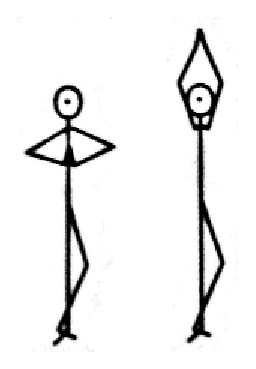
\includegraphics[width=2.3cm]{EqEx2}}\label{sf:equil} & 
First feel your center. Put {one foot on the other}. 

Put your {hands together} in front of you, then {lift them} slowly up; eventually lift your gaze, too.

Breathe very calmly and focus on your center.

Repeat on the other side.
  \\
   \raisebox{-0.8\totalheight}{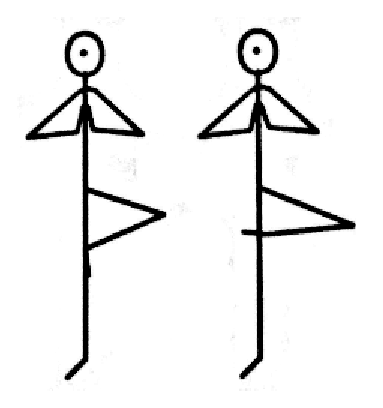
\includegraphics[width=2.7cm]{EqEx3}} & 
First feel your center. Take one {foot} 
and rest it against the {inner side of your knee}, if possible to your {thigh}.

Hold your hands in front of your sternum.

Breathe calmly. You can close your eyes. Breathe very calmly and focus on your center.

Repeat on the other side.
  \\
   \raisebox{-0.6\totalheight}{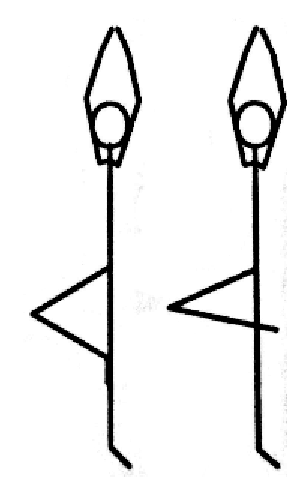
\includegraphics[width=1.9cm]{EqEx4}} & 
The same as before, but this time {raise your hands}. You can close your eyes.

Breathe calmly and focus on your center.

Repeat on the other side.

\end{tabular}


\end{document}